Using logic grid puzzles as a use-case, we will validate the feasibility of finding a sequence of small explanations.

As data we use puzzles from Puzzle Baron’s Logic Puzzles Volume 3~\cite{logigrammen}. The first 10 puzzles were used to construct the grammar. Using this grammar, and a semi-automatically problem-specific lexicon, we are able to parse and solve all puzzles in the booklet, including those not used to construct the grammar. Our experiments below are on test puzzles not used to construct the grammar; we also report results on the \textit{pasta} puzzle, which was emailed to us by a person that did not manage to solve it himself.\tias{do we know the source of the original puzzle?}

As constraint solving engine, we use IDP~\cite{idp}. It is a knowledge representation and reasoning system that supports multiple queries on a first order logic theory. We will use the 'optimalpropagate()' query, which efficiently finds the maximally consistent (partial) interpretation of a theory, which in our case is a full interpretation, e.g. the solution to the logic grid puzzle. We also use the 'findMUS()'\tias{Bart, how is it really name?} query that searches for a subset-minimal unsatisfiable core.

The algorithm itself is written in embedded LUA, which is provided as en imperative environment inside the otherwise declarative IDP system. The code was not optimized for efficiency and can at this point not be used in an interactive setting, as it takes between 15 minutes to a few hours to fully explain a logic grid puzzle. Experiments were run on an Intel(R) Xeon(R) CPU E3-1225 with 4 cores and 32 Gb memory, running linux 4.15.0 and IDP version 3.7.1.

\paragraph{1. Sequence composition}
We first look at the properties of the puzzles and the composition of the resulting sequence explanations. The results are shown in Table~\ref{table:composition}. Puzzle nr \tias{XXX} is the pasta puzzle. $|type|$ is the number of types of entities (e.g. person, sauce) while $|dom|$ is the number of entities of each type. $|grid|$ is the number of cells in the grid, e.g. the number of literals in the maximal consequence interpretation $I_n=max(I_0,\allconstraints)$.

Coincidentally, the puzzles all have 4 types with a domain of size 5, and hence 150 cells. We can see that the number of inference steps is around 120 for all but the pasta puzzle. When looking at the proportion of the inference steps that use bijections (only), transitivity (only) or a clue, we can see that around 50\% the explanations typically use a transitivity constraint, around 25\% typically a trivial bijectivity constraint (e.g. completing a row or column in one relation), and less then $1/5$th of the explanations actually need to use a clue.
In the table, \#m-i and \#m-c refer to the use of multiple implicit constraints and multiple clues respectively. We can see that it is never necessary to combine multiple constraints in one inference step. Also, notably, the puzzles from the booklet never require combining implicit constraints, while the anecdotically hard pasta puzzle is the only one that does, e.g. it can not be solved by focussing on the clues but one must combine facts and knowledge in the table alone to crack it.

\begin{table}
	\centering
	\resizebox{\columnwidth}{!}{%
\begin{tabular}{c|ccc|c|cccccc} 
	\hline
	n & $|type|$ & $|dom|$ & $|grid|$ & steps & \#bij & \#trans & \#clue & \#m-i & \#m-c \\ 
	\hline 
	p5 & 4 & 5 & 150 & 113 & 35 & 35 & 21 & 0 & 0\\ 
	\hline 
	p12 & 4 & 5  & 150 & 115 & 33 & 33 & 19 & 0 & 0\\ 
	\hline 
	p16 & 4 & 5 & 150 & 122 & 26 & 26 & 23 & 0 & 0\\ 
	\hline 
	p18 & 4 & 5  & 150 & 116 & 32 & 32 & 20 & 0 & 0\\ 
		\hline 
	p19 & 4 & 5  & 150 & 123 & 30 & 30 & 20 & 0 & 0\\ 
	\hline 
	p20 & 4 & 5  & 150 & 116 & 31 & 31 & 17 & 0 & 0\\ 
	\hline 
	nielspasta & 4 & 5  & 150  & 82 & 28 & 28 & 18 & 2 & 0\\ 
	\hline 
	p25 & 4 & 5  & 150 & 111 & 41 & 41 & 19 & 0 & 0\\ 
	\hline 
p93 & 4 & 5  & 150 & 119 & 40 & 40 & 22 & 0 & 0\\ 
\hline
\end{tabular}  
	}
\caption{Composition of puzzle explanations}
\label{table:composition}
\end{table}

\paragraph{2. Sequence progression}
Figure \ref{fig:steps} shows a visualisation the type of explanation used at every step of the sequence, for four different puzzles. The red line is the pasta puzzle. We can see that typically at the beginning of the sequence, clues (4th line) and bijectivity (2nd line) are used, e.g. the trivial ones. This is then followed by a round of clues and some bijectivity/transitivity, after which a large fraction of the table can be completed with bijectivity/transitivty, followed by a few last clues and another round of completion.

The exception to this is the paste puzzle. We can see that after around 20 steps where mostly clues have been used, twice a combination of implicit logigram constraints must be used to derive a new fact, after which the table can be easily completed with bijectivity/transitivity and twice the use of a clue.
\tias{Ideally, the 0th row is start/end and the line both starts and ends there (e.g. no 'solution' top line), will also help in readability/space usage}

\begin{figure}
\centering
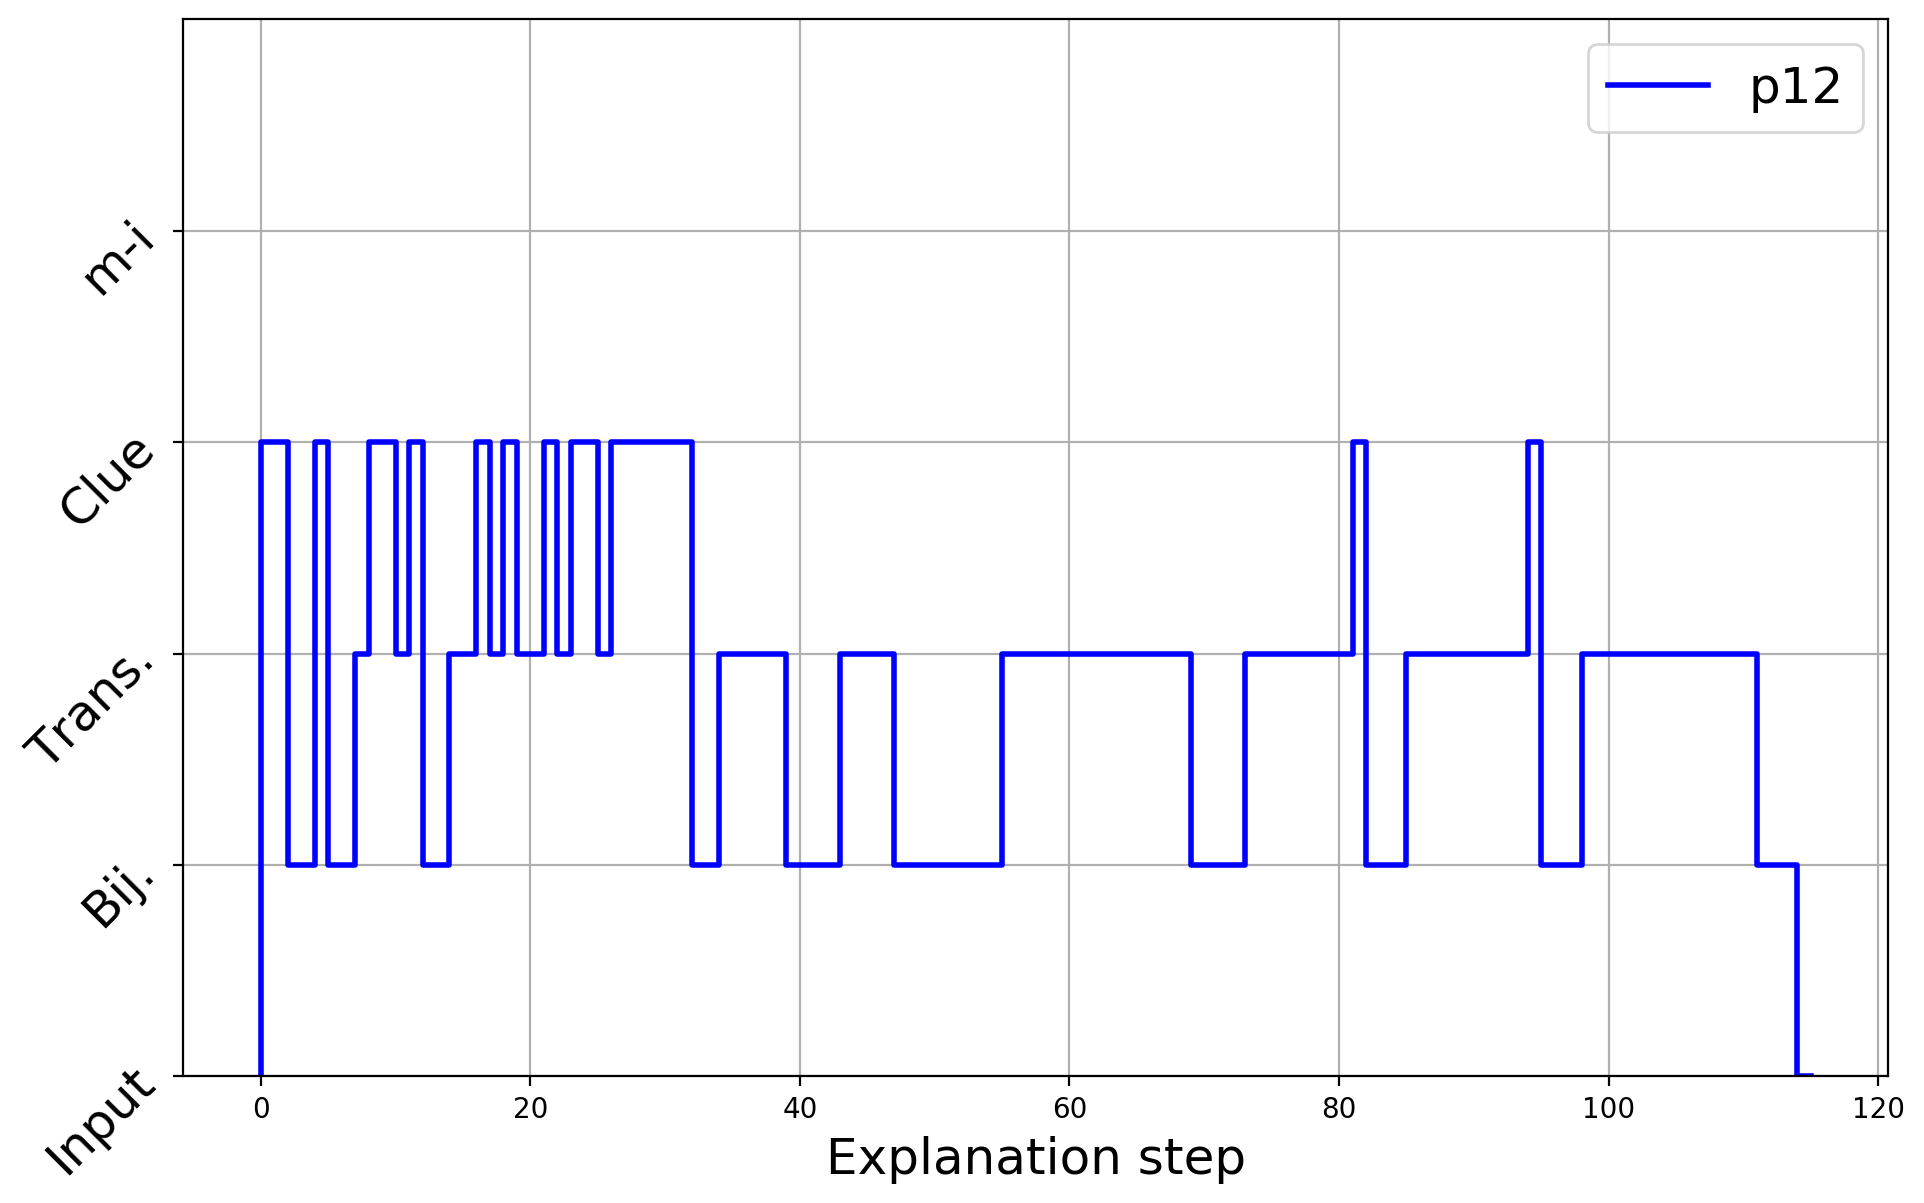
\includegraphics[width=0.49\linewidth]{figures/plot_cost_steps_p12}
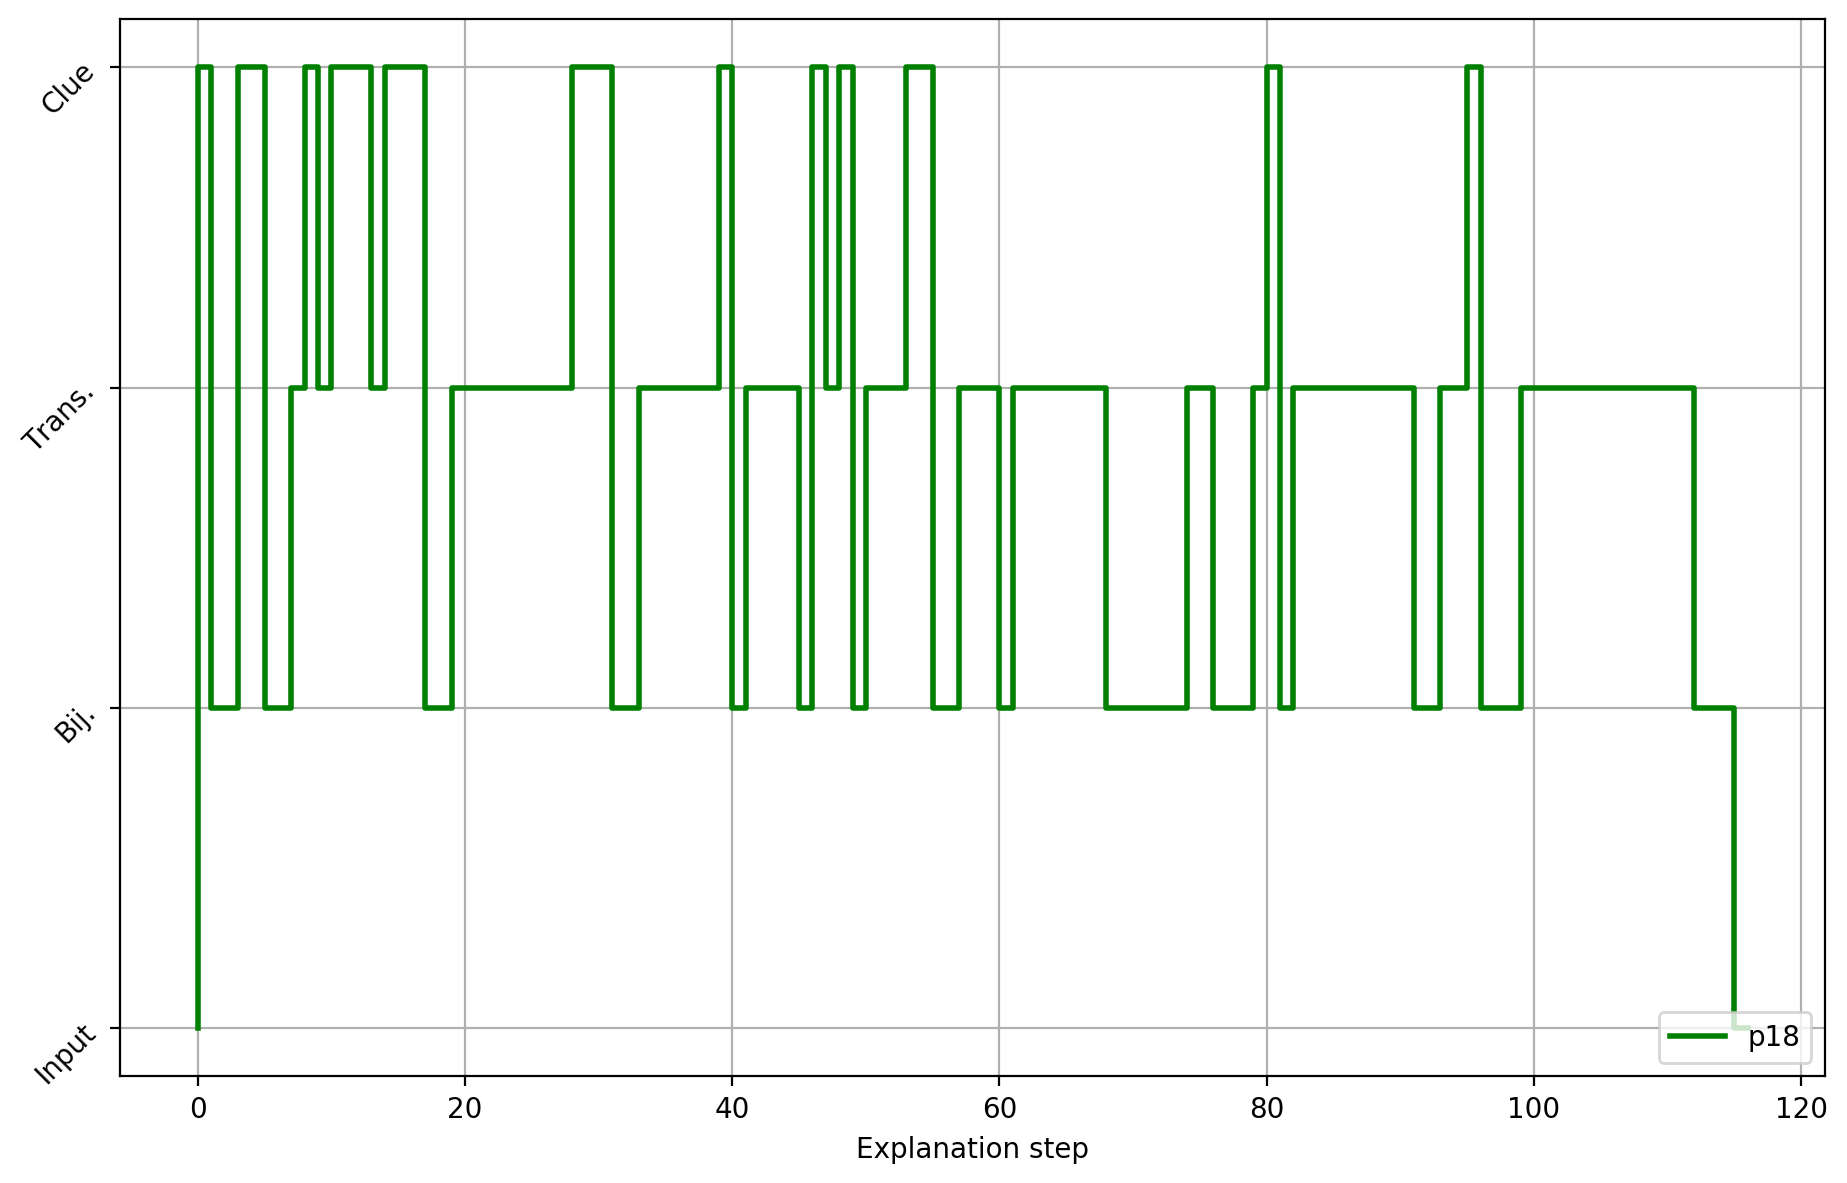
\includegraphics[width=0.49\linewidth]{figures/plot_cost_steps_p18}
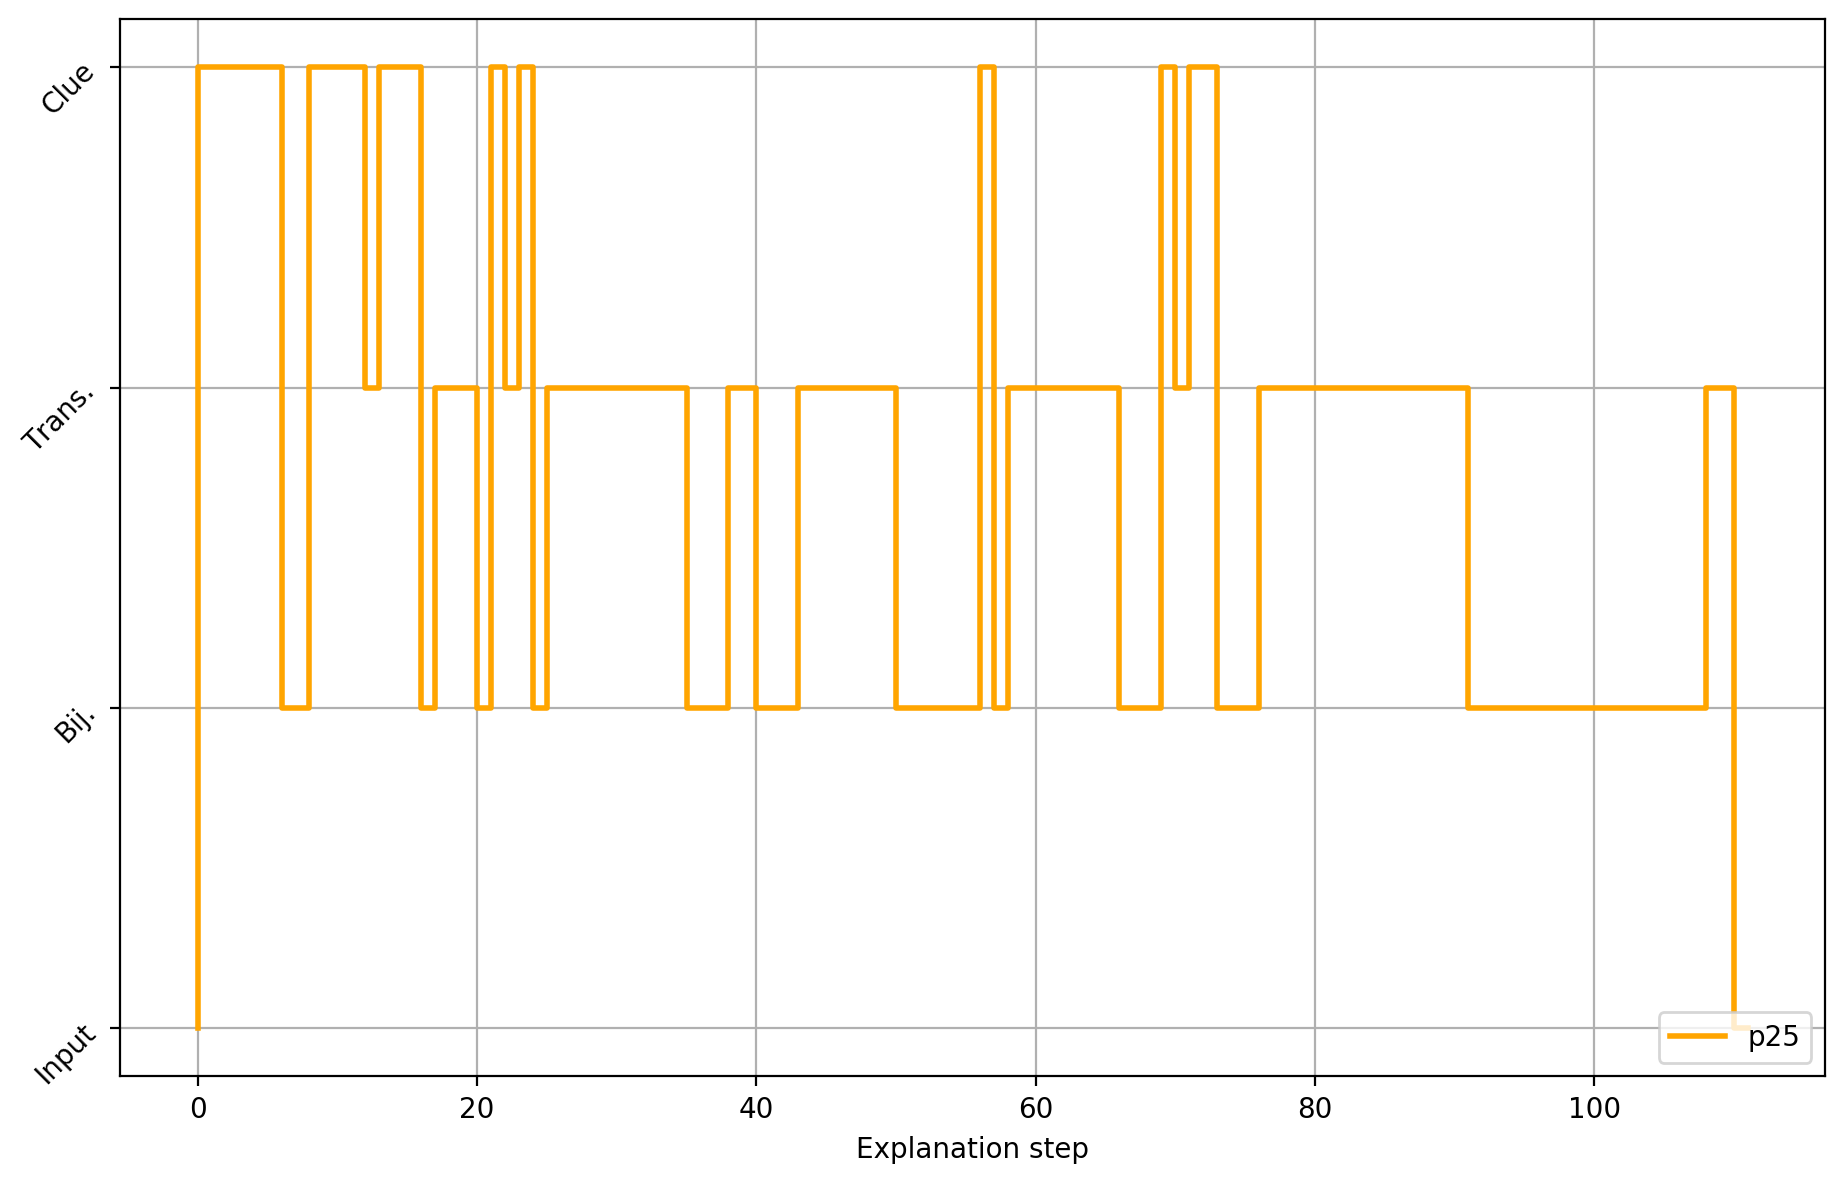
\includegraphics[width=0.49\linewidth]{figures/plot_cost_steps_p25}
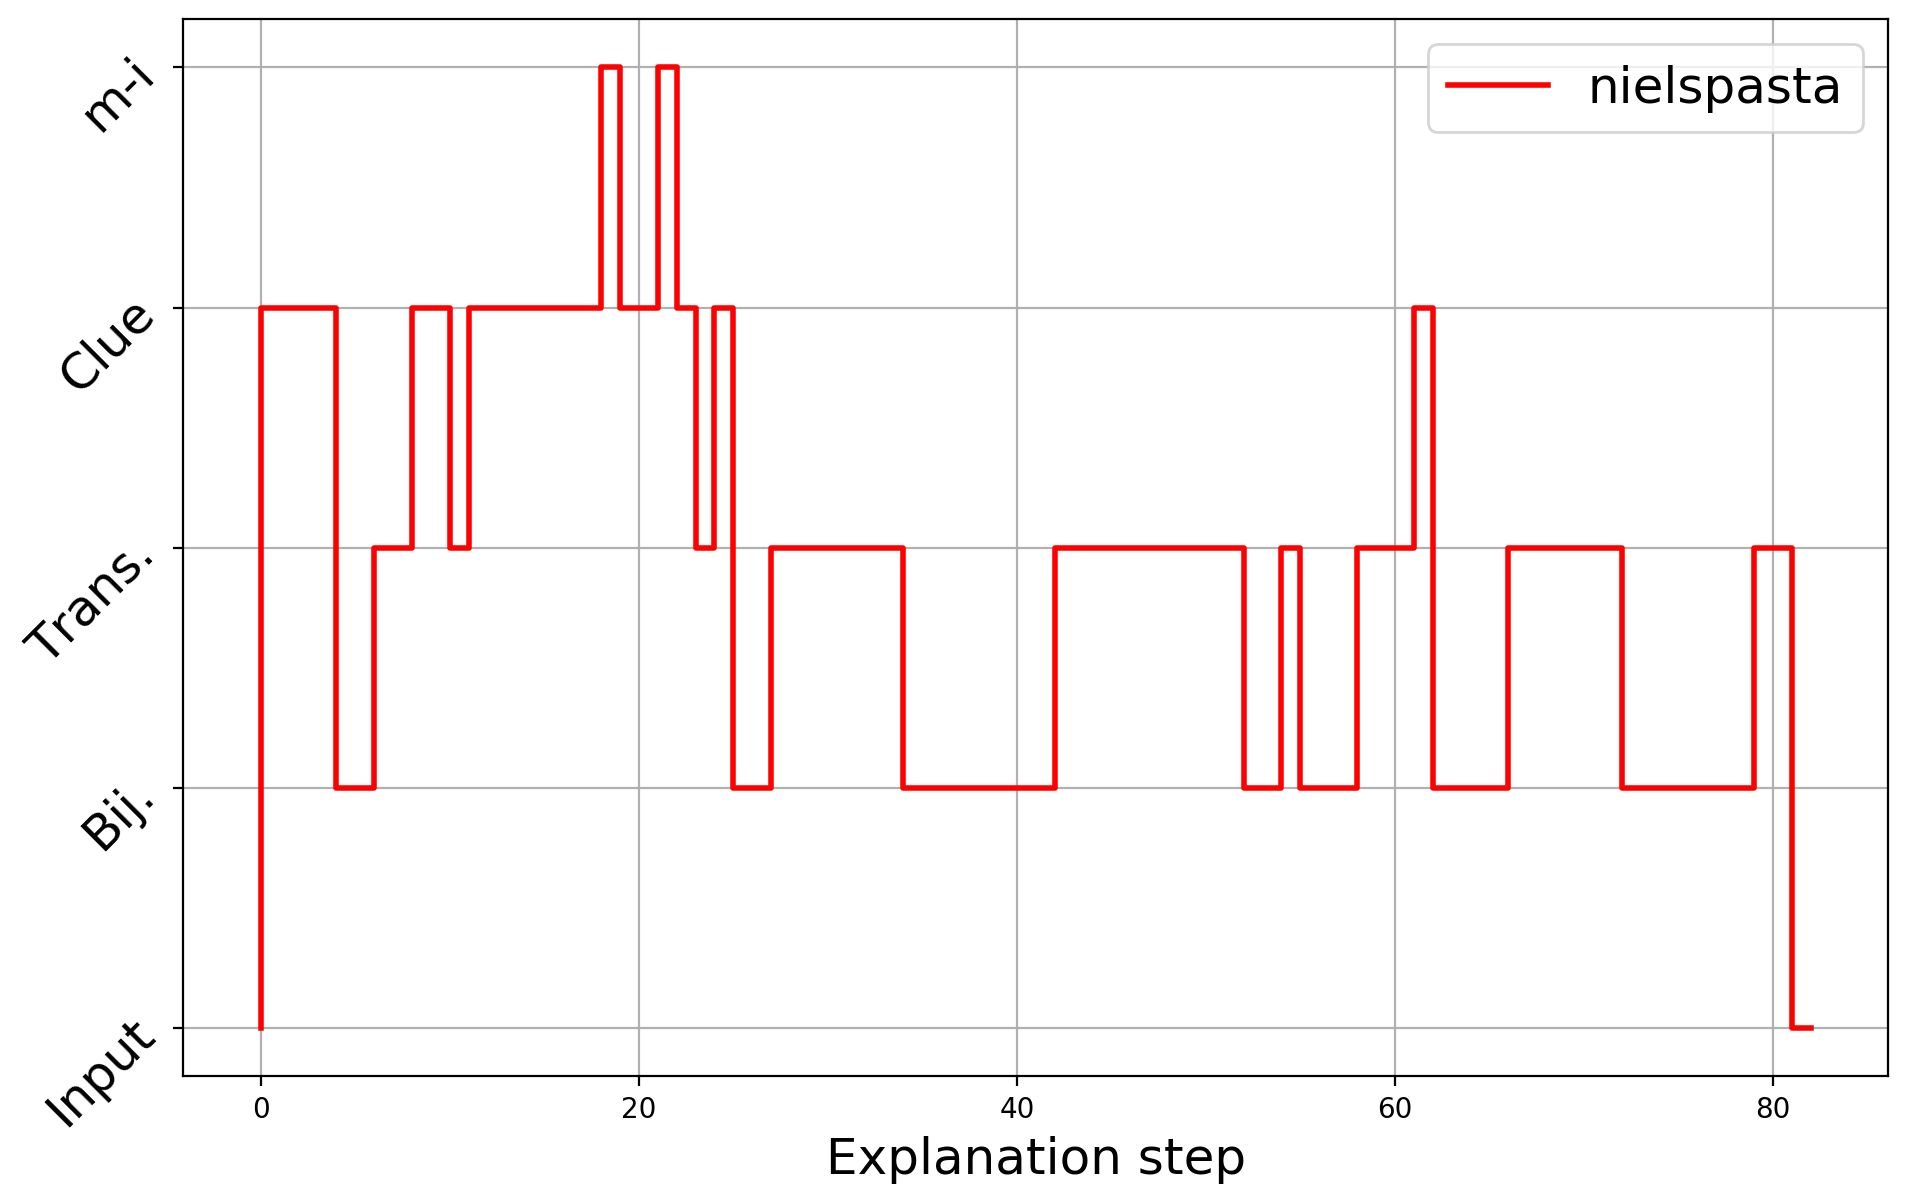
\includegraphics[width=0.49\linewidth]{figures/plot_cost_steps_nielspasta}
\caption{}
\label{fig:steps}
\end{figure}



While the first part of the table \ref{table:sequence_leve} only analyzes the difficulty of a puzzle, the second part focuses on the explanations. 
Most of the explanations are either generated using bijectivity (bij.) or Transitivity (trans.). The rest are found using the 1 or more clues, or by combining (comb.) transitivity with bijectivity. This is due to the way puzzles are formulated in natural language for logic grid puzzles.

\paragraph{Q2. How does the level of difficulty progress throughout the explanation?} Out of the problems in table \ref{table:sequence_leve}, 3 puzzle instances were selected: \textit{p12}, \textit{p18} and \textit{p25}. These puzzles present a similar number of explanation steps and total costs.

\begin{figure}
	\centering
	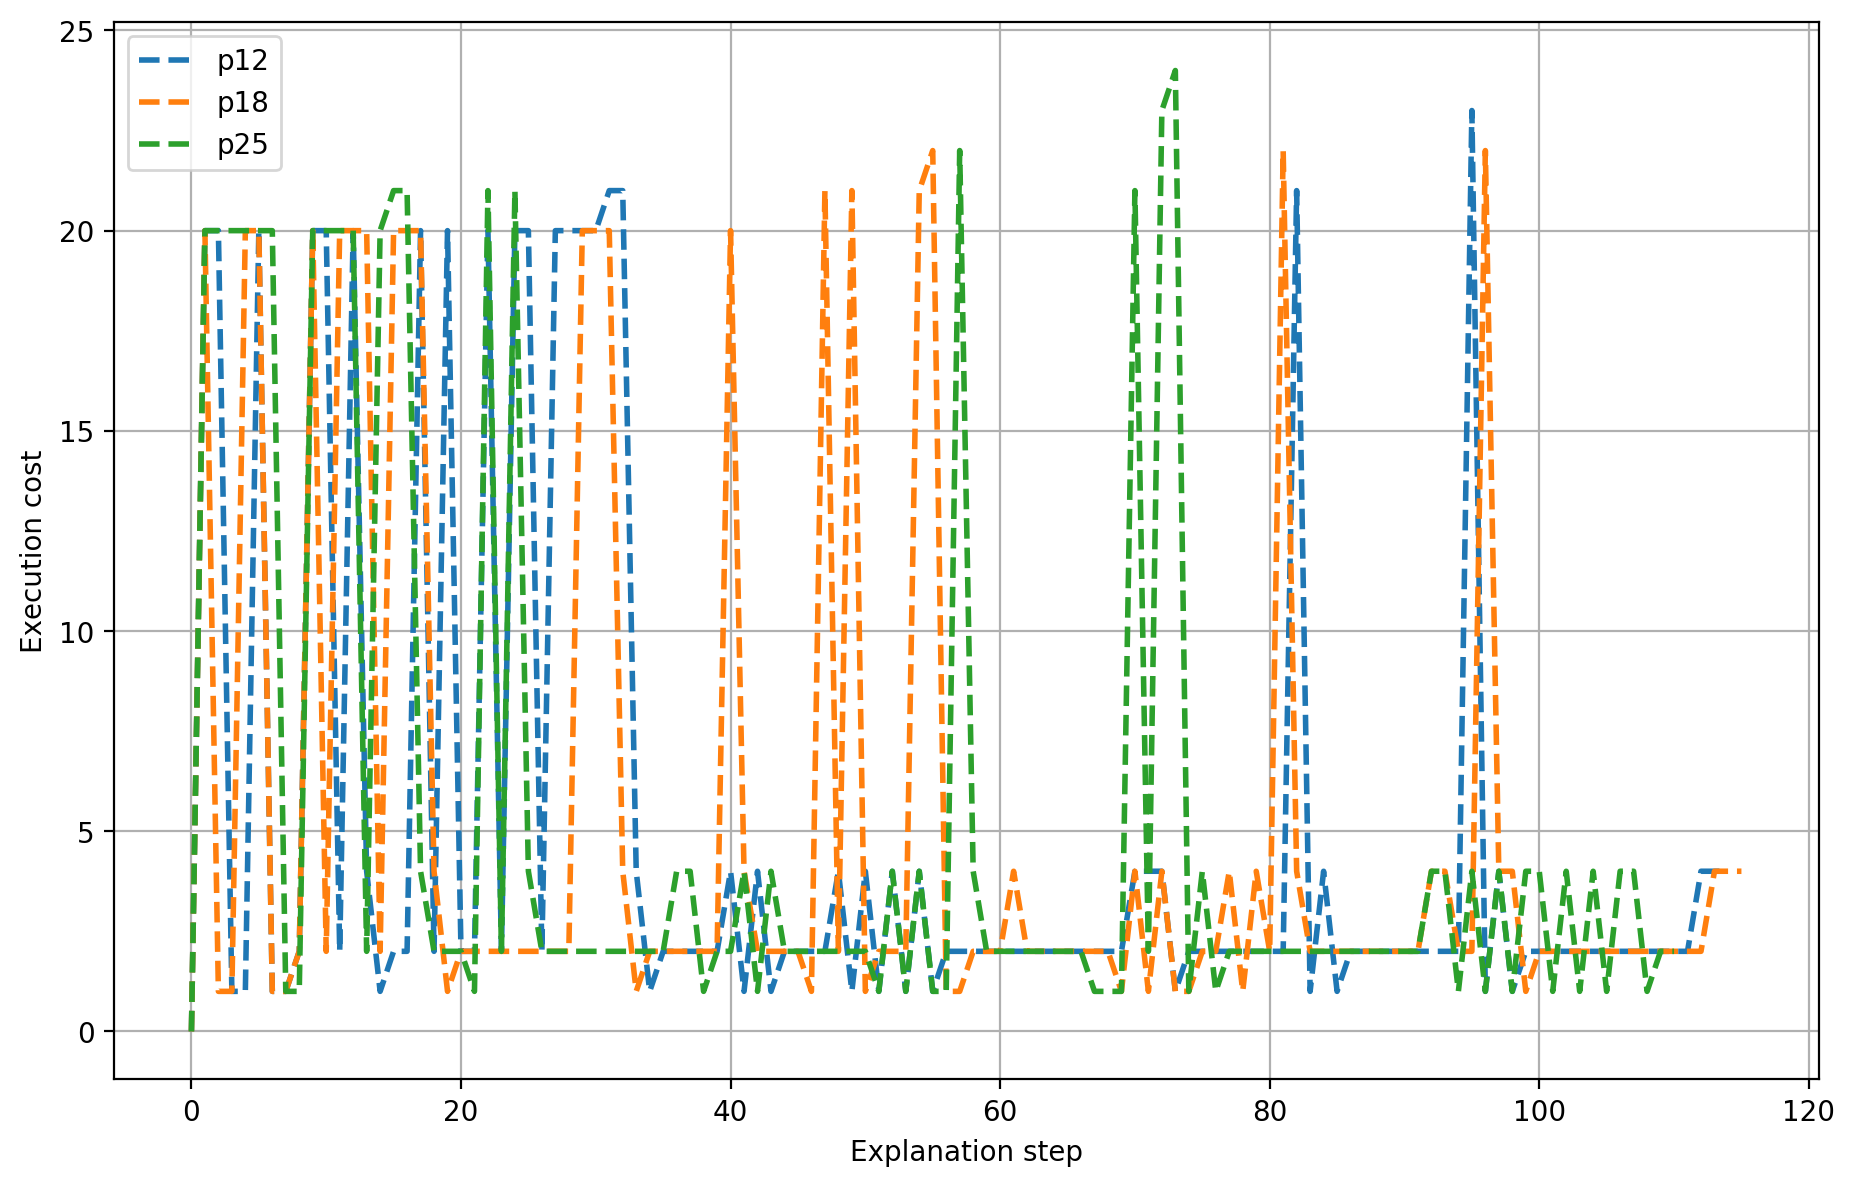
\includegraphics[width=0.7\linewidth]{figures/plot_cost_steps.png}
		\caption{Explanation cost for puzzle instances p12, p18, p25}
			\label{fig:plotcoststeps}
\end{figure}

\begin{table}
	\centering
	\resizebox{\columnwidth}{!}{%
		\begin{tabular}{|l||c|c|c|c|c|c|c|} 
			\hline
			\textbf{puzzle} & \textbf{tot exec time} & avg clue time  & avg bij. & avg trans. & avg time/cost of clue & avg time/cost of bij. & avg time/cost of bij. \\ 
			\hline 
			p5 & 386.0 & 129.29 & 226.27 & 204.23 & 6.13 & 145.18 & 102.11 \\ 
			\hline 
			p16 & 576.0 & 192.97 & 370.55 & 426.41 & 9.22 & 213.63 & 213.21 \\ 
			\hline 
			p93 & 946.0 & 213.13 & 604.13 & 425.58 & 10.44 & 340.27 & 212.79 \\ 
			\hline 
			p12 & 1103.0 & 271.13 & 744.93 & 799.79 & 12.87 & 432.21 & 399.89 \\ 
			\hline 
			p18 & 1924.0 & 323.82 & 856.52 & 881.44 & 15.14 & 421.34 & 440.72 \\ 
			\hline 
			p20 & 411.0 & 117.57 & 235.34 & 235.29 & 5.69 & 147.65 & 117.64 \\ 
			\hline 
			p25 & 886.0 & 291.12 & 659.88 & 623.77 & 13.42 & 404.61 & 311.89 \\ 
			\hline 
			p19 & 1207.0 & 265.82 & 538.64 & 602.01 & 12.77 & 293.38 & 301.0 \\ 
			\hline 
		\end{tabular} 
	}
	\caption{Puzzle explanation cost based on the cost function $f(I, C)$ and statistics on puzzle constraints}
	\label{table:sequence_leve}
\end{table}


\paragraph{Q3. How is the performance and the level of difficulty affected by removing parts of the algorithm ? } bla bla bla

% TODO table : Leaving some parts of the algo out, to see step-wise improvements of the components?  Some experiment with different levels of abstraction (e.g. all constraints at once, clues separate but all implicit at once, 2 groups of implicits, full split of implicits) with 'set of measures', so probably a table

\paragraph{Bonus. How well does it compare to human solving process ?} 

% TODO Compare with the tutorial puzzle of logicgridpuzzles.com? Ideally, a small human evaluation (e.g. ask people to solve a 3-with-3 puzzle and note the order of derivations and clues used, compare this 'ranking' to our ranking, discuss some differences.

\begin{table}
	\centering
	\resizebox{\columnwidth}{!}{%
		\begin{tabular}{|l||c|c|c|c|} 
			\hline 
			\textbf{puzzle} & \textbf{avg. fact used} & \textbf{avg. facts used with a clue} & \textbf{avg. facts used with trans.} & \textbf{avg. facts used together with bij.}\\ 
			\hline 
			p5 & 1.823 & 0.524 & 2.371 & 2.0 \\ 
			\hline 
			p16 & 1.803 & 0.609 & 2.385 & 2.0 \\ 
			\hline 
			p93 & 1.84 & 0.182 & 2.575 & 2.0 \\ 
			\hline 
			p12 & 1.835 & 0.316 & 2.455 & 2.0 \\ 
			\hline 
			p18 & 1.853 & 0.45 & 2.5 & 2.0 \\ 
			\hline 
			p20 & 1.828 & 0.294 & 2.355 & 2.0 \\ 
			\hline 
			nielspasta & 1.768 & 1.05 & 2.071 & 2.0 \\ 
			\hline 
			p25 & 1.937 & 0.737 & 2.463 & 2.0 \\ 
			\hline 
			p19 & 1.87 & 0.4 & 2.6 & 2.0 \\ 
			\hline 
		\end{tabular} 
	}
	\caption{Puzzle explanation cost based on the cost function $f(I, C)$ and statistics on puzzle constraints}
	\label{table:sequence_leve}
\end{table}

